\chapter{Overview}
\label{overview}

This chapter provides an overview of \name. We first elaborate the fundamental goals
of this research, along with requirements, and design choices (\S\ref{sec:design}).
We then outline \name including a brief introduction of each component and their
workflow (\S\ref{sec:overview}). Finally, we describe our threat model
(\S\ref{sec:threatmodel}) and state our assumptions (\S\ref{sec:assumptions}).

\section{Design Principles}
\label{sec:design}

\paragraph{Goal}
The fundamental goal of this work is to build an architecture that combines local
network zoning and inter-domain routing with regard to secure zone transfers, lightweight protocol interoperability,
and incremental deployability---thereby enabling secure,
scalable, and flexible network zoning on a global scale. That is, an administration
domain expresses zone definitions and corresponding zone transfer rules, and
deploys the policies to distributed network entities. These policies force the
network to only forward authorized packets protected by cryptographically
secured authenticators, ensuring secure and sustainable zone-to-zone communication.

\paragraph{Desired Properties}
We consider the following properties to achieve this goal.

\begin{itemize}
	% \item Strong security guarantee: the zone transfer protocol applies strong
	% cryptography primitives, such that no security sensitive information is exposed 
	% while the data is being transmitted via the public Internet. 
	\item Data confidentiality: through a constructive approach, the zone transfer
	      protocol ensures that no information
	      is exposed while being transmitted via the public Internet.
	\item Management scalability: logically centralized orchestration empowers
	      network administrators to easily migrate network topologies, update policies and
	      mirror abstract network zones into the real network.
	      % \item Practicality: the modern cryptographic primitives that we use are 
	      % lightweight, such that they do not introduce severe performance overheads in terms of 
	      % latency, bandwidth, and operational costs.
	\item Efficiency: the cryptographic primitives introduce only minor performance
	      overhead in terms of latency, bandwidth, and operational costs.
	\item Deployability: the \name architecture requires minimal changes to the
	      existing network infrastructure in order to achieve compatibility. Furthermore,
	      firewalls and VPN devices
	      at each entry point of every zone can be replaced with one \name gateway, saving
	      operational costs for the same level of network security.
\end{itemize}


\paragraph{Design Choices}
% We design \name working with mature technologies that are well embraced in 
% modern the Internet environment, such that our architecture keeps its practicality 
% and deployability. In particular, the following design choices are considered:
We design \name working with mature technologies that are embraced in modern enterprise
environments. In particular, the following design choices are made:

\begin{itemize}
	\item Network programmability is realized with the concept of a logically centralized
	      controller (e.g., SDN), preserving management flexibility and scalability.
	\item Asymmetric cryptography is used for core operations where source
	      authenticity is critical (e.g., symmetric key exchange).
	\item Symmetric cryptography is used for the rest of the data
	      transmission, ensuring efficient packet processing.
\end{itemize}

\begin{figure}[htb]
	\begin{center}
		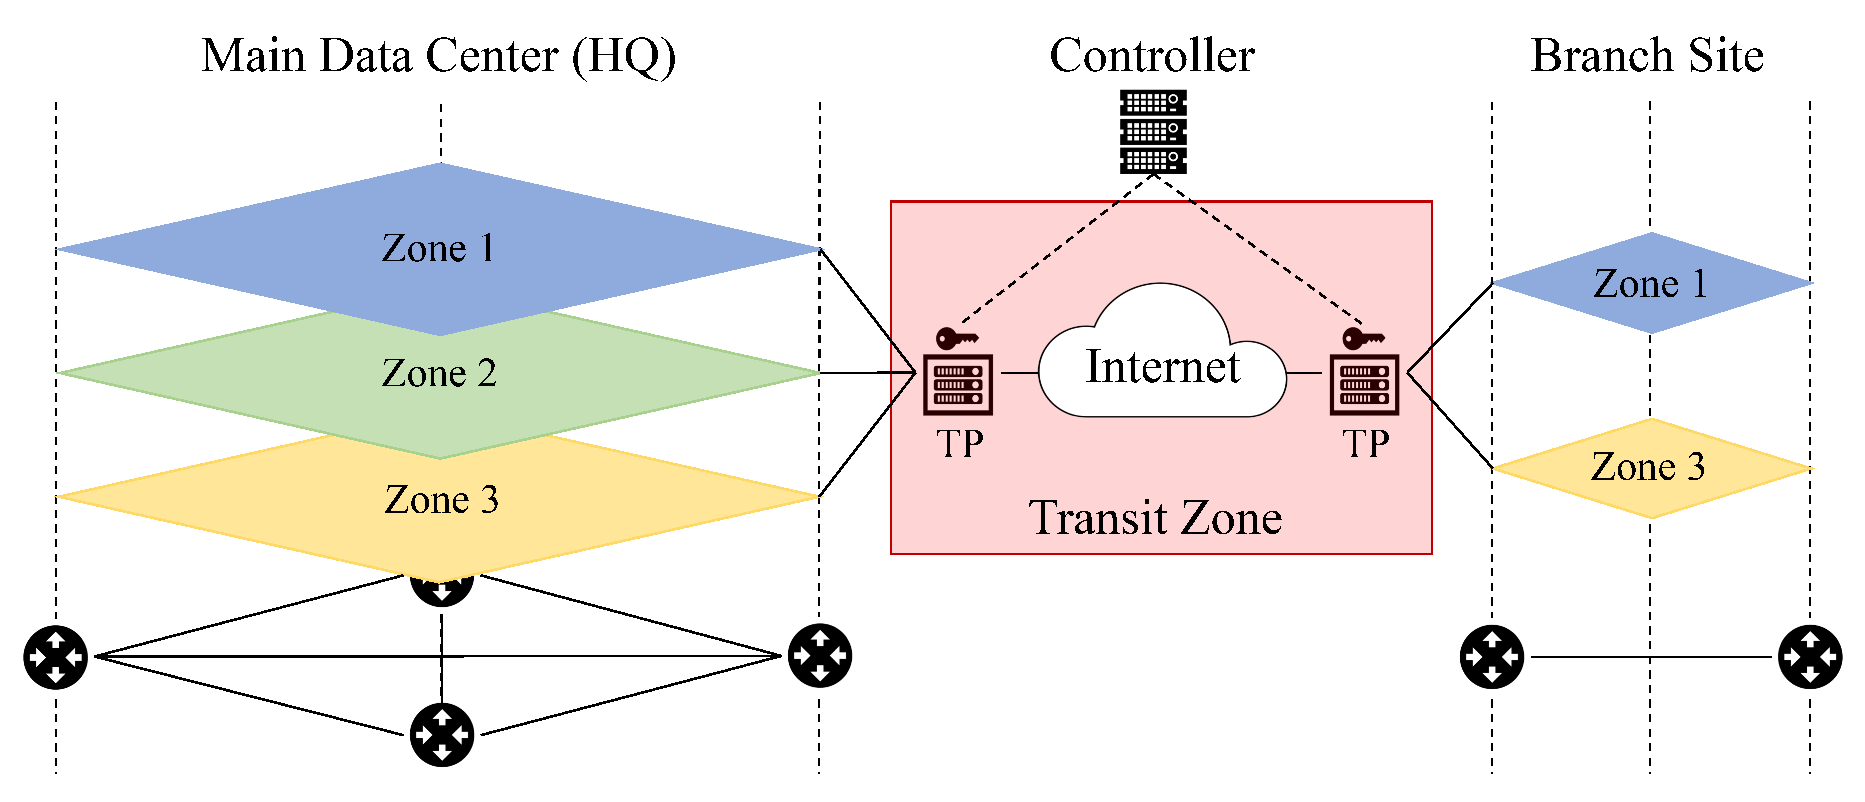
\includegraphics[width=.9\textwidth]{overview.eps}
	\end{center}
	\caption{An overview of the \name architecture. The inter-domain transit zone interconnects physically
		and logically distributed network zones with unified security policy enforcement.}
	\label{fig:overview}
\end{figure}

\section{\name Overview}
\label{sec:overview}

\paragraph{Entities in \name}
Figure~\ref{fig:overview} illustrates an overview of \name.
Different branch sites of an enterprise are interconnected over a WAN (\eg the Internet). Each site
contains multiple, logically separated zones connected to the single zone
Translation Point (\tp) at the corresponding site. The \tp is a designated gateway
for zone transfers, operating on layer 3 and interconnecting all zones at a given
site of the enterprise network. All the traffic towards either internal network or
WAN, therefore, passes through the \tp. Note that \tps are the endpoints
of our architecture, meaning that everything beyond that point should not be
modified for ease of deployment and to ensure compatibility with the modern enterprise
environments.

\begin{floatingfigure}[r]{0.69\linewidth}
	\centering
	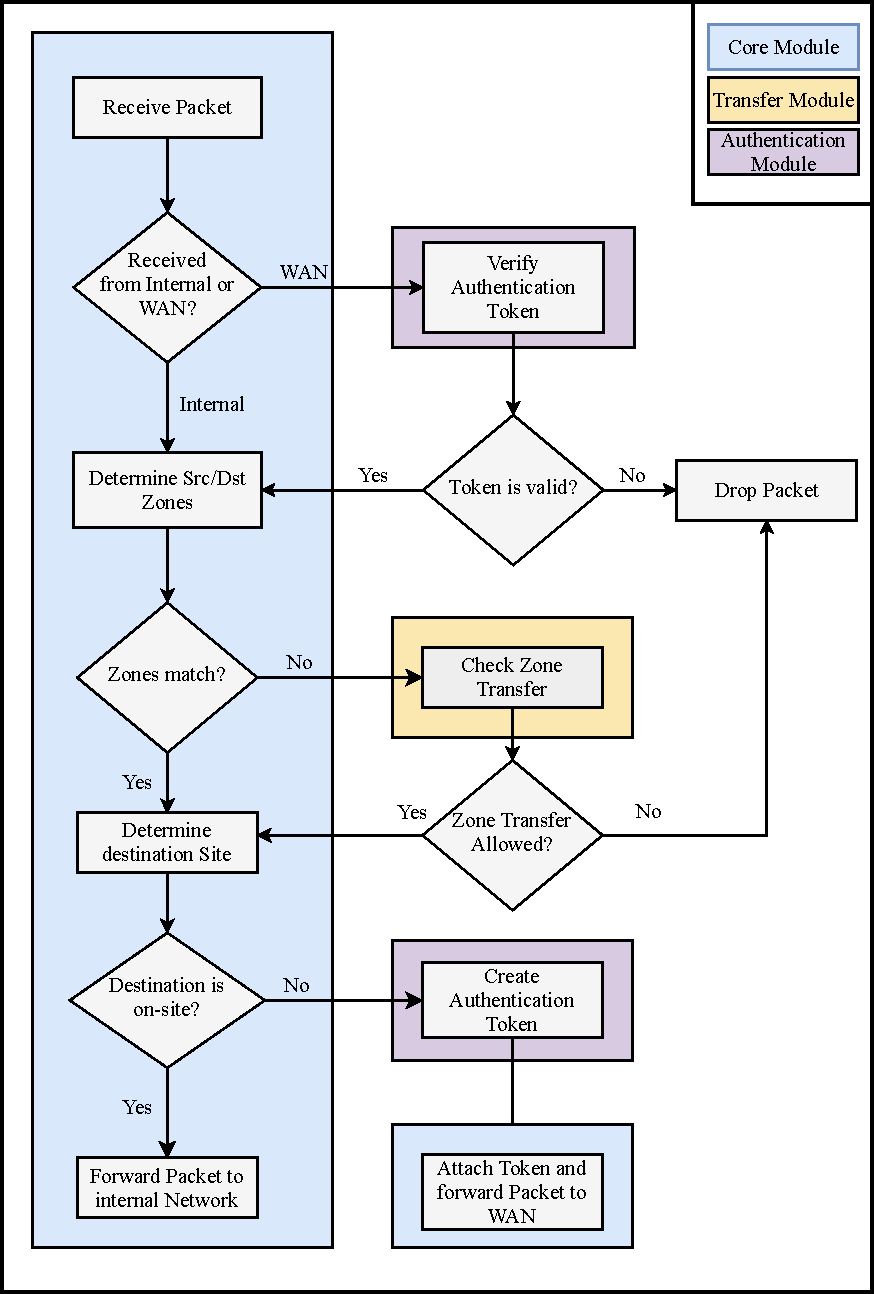
\includegraphics[width=.65\linewidth]{tp_controlflow.pdf}
	\caption{Control flow of the zone Translation Point.}
	\label{fig:flow}
\end{floatingfigure}

The main task of \tps is twofold: first, they ensure that traffic adheres to a
set of allowed zone transitions. For a packet originating in a zone and destined
for another zone, the transition must be explicitly allowed by a policy. Second,
\tps enable communication across the WAN without losing previously established
security information. To this end, \tps embed an authentication token with
cryptographically secured zone information into packets before they leave the
internal network. Furthermore, \tps act as endpoints hiding sensitive
information, such as internal addresses and the respective zone binding, from
external entities. We also note that, for a case where zones with the same
security requirements and functionality are distributed over multiple branch
sites (e.g., Zone 1 and 3 in Figure~\ref{fig:overview}), we consider them as the
same logical zone (e.g., the same zone identifier). We call this concept zone
extension which is not subject to zone authorization.

A logically centralized controller orchestrates the \tps. The controller is owned
by a single administration domain, and thus the owner of the controller owns all
the zones behind the \tps. The controller provides its owner a management interface
in which the owner designs an outline of zone structure and transfer policies. The
explicit network configuration is then distributed to the \tps via a secure control
channel to enforce the configuration at the individual premises.

\paragraph{Communication Flow}

\name enables secure zone transfers over WAN as follows:

\begin{enumerate}
	\item Network administrators first establish an IP-zone map and their transfer
	      policies, which represents a virtual network configuration that explicitly
	      specifies reachability, and upload them to the logically centralized
	      controller.
	\item Each pair of \tps exchanges symmetric keys to establish a secure tunnel.
	      The key is being updated frequently through a state-of-the-art key management and
	      distribution system that protects the secrecy of the zone transfer from
	      being exposed to the public while ensuring high-speed data transmission.
	\item The on-site \tp inspects all the packets to be transmitted to another zone.
	      The \tp acquires the corresponding zone transfer policy from the controller
	      and verifies if the transmission is authorized.
	\item If a packet is authorized, the \tp looks up the respective end-point \tp,
	      encrypts the packet along with the corresponding zone transfer information,
	      and forwards it across the WAN. Otherwise, the packet is dropped.
	\item The remote-site \tp then decrypts the packet and forwards it according to
	      the enclosed zone transfer information. The receiving \tp could also verify
	      the validity of the packet transmission if desired.
\end{enumerate}

Figure~\ref{fig:flow} shows the control flow of a \tp.

\section{Threat Model}
\label{sec:threatmodel}
We consider a threat model in which attackers reside either on-premise (i.e., compromised
end hosts) or are located
outside of the cooperative networks. The goal of attackers is to access unauthorized zones
to exfiltrate information assets, or disrupt networks and services. To achieve this goal,
attackers can use the following strategies:

% \paragraph{Reconnaissance}
% % Attackers can observe or collect legitimate network traffic at "Checkpoint 
% % Charlie"---aggregation points where the zone transfer packets traverse---to map the
% % pairs of hosts and their corresponding security policies. For instance, tapping the
% % wire near entry points of enterprise networks is feasible. 
% Attackers can observe or collect legitimate network traffic at aggregation points through 
% which the zone transfer packets traverse, to map the
% pairs of hosts and their corresponding security policies. For instance, by eavesdropping
% near entry points of enterprise networks. 

\paragraph{Unauthorized Access}
Attackers may disguise as authorized entities to blind the security middleboxes and
access restricted zones.
% We have witnessed that impersonating other network entities 
% is a common attack scheme in many network systems. \ml{Is there something to reference?} 
A more sophisticated attack is to override security systems by directly injecting
tampered policies.

\paragraph{Denial-of-Service}
Here, the goal is to disrupt the target networks or services. Attackers can sabotage the core network
systems, for example, by flooding security middleboxes that perform deep packet inspection.
This might then lead to network performance degradation, causing
denial-of-service for legitimate clients.

% \paragraph{Exfiltration}
% Sensitive and business-critical data is stolen and forwarded to a remote server on the
% attacker's premises. In most cases, the data is stored in the restricted zones with 
% the highest level of trust---establishing a communication channel from highly trusted
% zones to a low-level zone is commonly not constrained---attackers can easily exfiltrate
% the highly valuable information assets. \claude{I don't understand this scenario. How does the attacker get access to a high security zone?} \jk{This is an attacker model after succeeding 
% infiltration to the high secure zone. Nonetheless, we'd better not to describe this anyway.}

% In our threat model, we assume that components of \name (i.e., \tps and controllers) 
% are resilient against compromise attacks, and therefore trustworthy.


\section{Assumptions}
\label{sec:assumptions}

\paragraph{Public Key Infrastructure}
A given enterprise network has a public key infrastructure (PKI). That is, the
enterprise creates a trust model for its network infrastructure, acts as a
trusted certificate authority (CA), and issues certificates for the core
systems. Entities can retrieve and verify the public keys of the core systems.
There are open source projects, such as
\fnurl{EJBCA}{https://svn.cesecore.eu/svn/ejbca/trunk/ejbca/} and
\fnurl{OpenXPKI}{https://github.com/openxpki/openxpki/}, available for setting
up enterprise-grade PKIs.

\paragraph{Secure Cryptography}
Cryptographic primitives we use in \name are secure; authenticity, integrity, and
confidentiality remain intact unless the cryptographic keys are exposed.

\paragraph{Time Synchronization}
Core entities within the cooperative network have loosely synchronized system clocks with a
precision of seconds (e.g., network time protocol achieves a precision of tens of milliseconds).
Time synchronization is mainly used to constrain the validity of cryptographic keys.

\paragraph{Sole Administration}
A network has a sole administration domain (e.g., enterprise) which has full control over
the network architecture and security policy. To access the network, collaborators
must obey this policy.
